% Source: AESP_466_ClassWork/Supplements/Notes/latex/6.6/6.6.tex

\documentclass[border=4pt]{standalone}
\usepackage{amsmath,amssymb,amsthm}
\usepackage{graphicx}
\usepackage{tikz}
\usepackage{xcolor}
\usetikzlibrary{arrows.meta,calc,positioning,decorations.markings,patterns,shapes.geometric,angles,quotes}

\definecolor{Garnet}{HTML}{73000A}
\definecolor{USC_Rose}{HTML}{CC2E40}
\definecolor{USC_Blue}{HTML}{466A9F}
\definecolor{USC_Slate}{HTML}{1F414D}
\definecolor{USC_Olive}{HTML}{65780B}
\definecolor{USC_Lime}{HTML}{CED318}
\definecolor{USC_Gold}{HTML}{A49137}
\definecolor{USC_Black90}{HTML}{565556}
\definecolor{USC_Black10}{HTML}{ECECEC}

\newcommand{\vect}[1]{\mathbf{#1}}
\newcommand{\mat}[1]{\mathbf{#1}}
\newcommand{\uvec}[1]{\hat{\mathbf{#1}}}
\newcommand{\transpose}{^{\mkern-1.5mu\mathsf{T}}}
\newcommand{\inv}{^{-1}}
\newcommand{\deriv}[2]{\frac{d #1}{d #2}}
\newcommand{\pderiv}[2]{\frac{\partial #1}{\partial #2}}

\begin{document}
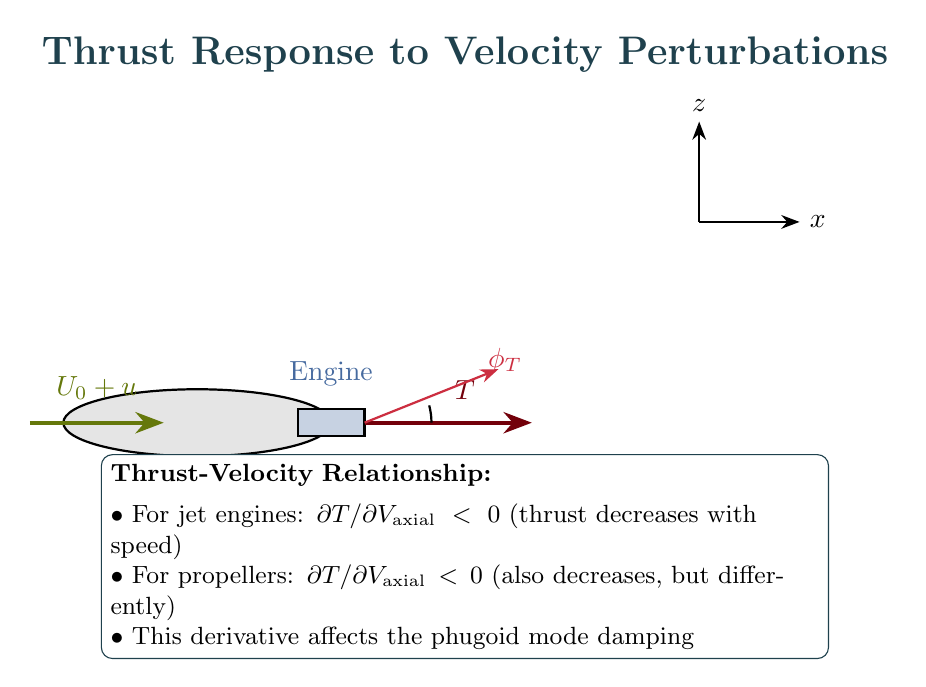
\begin{tikzpicture}[>=Stealth, scale=0.85]
    % Title
    \node[font=\Large\bfseries, USC_Slate] at (5,5.5) {Thrust Response to Velocity Perturbations};

    % Aircraft body
    \draw[thick, fill=gray!20] (1,0) ellipse (2 and 0.5);

    % Engine/thrust
    \draw[thick, fill=USC_Blue!30] (2.5,-0.2) rectangle (3.5,0.2);
    \node[USC_Blue, above] at (3,0.4) {Engine};

    % Thrust vector
    \draw[->, ultra thick, Garnet] (3.5,0) -- (6,0);
    \node[Garnet, above] at (5,0.2) {$T$};

    % Velocity vector
    \draw[->, ultra thick, USC_Olive] (-1.5,0) -- (0.5,0);
    \node[USC_Olive, above] at (-0.5,0.2) {$U_0 + u$};

    % Thrust angle
    \draw[->, thick, USC_Rose] (3.5,0) -- (5.5,0.8);
    \node[USC_Rose, above right] at (5.2,0.6) {$\phi_T$};
    \draw[thick] (4.5,0) arc (0:15:1);

    % Annotation box
    \node[draw=USC_Slate, fill=white, rounded corners, align=left, font=\small, text width=9cm] at (5,-2) {
        \textbf{Thrust-Velocity Relationship:}\\[4pt]
        $\bullet$ For jet engines: $\partial T/\partial V_{\text{axial}} < 0$ (thrust decreases with speed)\\
        $\bullet$ For propellers: $\partial T/\partial V_{\text{axial}} < 0$ (also decreases, but differently)\\
        $\bullet$ This derivative affects the phugoid mode damping
    };

    % Axes
    \draw[->, thick] (8.5,3) -- (10,3) node[right] {$x$};
    \draw[->, thick] (8.5,3) -- (8.5,4.5) node[above] {$z$};

\end{tikzpicture}
\end{document}
